\documentclass[a4paper,12pt]{article}
\usepackage{amsmath}
\usepackage{amssymb}
\usepackage{graphicx}
\usepackage{geometry}
\usepackage{hyperref}

\usepackage[slovene]{babel}
\usepackage[T1]{fontenc}
\usepackage[utf8]{inputenc}
\setlength{\parindent}{0pt} % lahko odstraniš, mene so sam malo motili zamiki

\geometry{margin=2.5cm}

\begin{document}

\title{$n$-kratno nihalo}
\author{Nena Šefman Hodnik, Nina Švigelj}
\date{}
\maketitle


\section{Dvojno nihalo}

Oglejmo si primer na sliki:

\begin{figure}[h!]
    \centering
    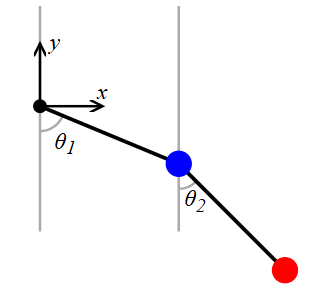
\includegraphics[width=0.3\textwidth]{primer_dveh_slika.png}
    \caption{Vir slike: \url{https://scipython.com/blog/the-double-pendulum/}}
    \label{fig:dvojno_nihalo}
\end{figure}

Imamo dve žogici z masama $m_1$ in $m_2$ na palčkah dolžine $l_1$ in $l_2$ z zanemarljivo maso.

Recimo, da je prva žogica na $(x_1, y_1)$ in druga žogica na $(x_2, y_2)$. Te koordinate dobimo kot:
\begin{align*}
x_1 &= l_1 \sin(\theta_1), \\
x_2 &= l_1 \sin(\theta_1) + l_2 \sin(\theta_2), \\
y_1 &= -l_1 \cos(\theta_1), \\
y_2 &= -l_1 \cos(\theta_1) - l_2 \cos(\theta_2).
\end{align*}

\subsection*{Potencialna energija}

Potencialna energija je definirana kot $V = m g h$, kjer je višina žogice dana z $h = y$. \\
Za posamezni masi velja: $$h_1 = y_1, \quad h_2 = y_2.$$

Torej celotna potencialna energija sistema je:
\begin{align*}
V &= V_1 + V_2 \\
&= m_1 g(-l_1 \cos\theta_1) + m_2 g(-l_1 \cos\theta_1 - l_2 \cos\theta_2).
\end{align*}

\subsection*{Kinetična energija}

Kinetična energija vsake žogice je podana z izrazom $$T = \frac{1}{2} m v^2.$$

Hitrost žogic dobimo s pomočjo izraza $v = \sqrt{\dot{x}^2 + \dot{y}^2}$.

Odvodi koordinat so: \begin{align*}
\dot{x}_1 &= l_1 \dot{\theta}_1 \cos(\theta_1) \\
\dot{x}_2 &= l_1 \dot{\theta}_1 \cos(\theta_1) + l_2 \dot{\theta}_2 \cos(\theta_2) \\
\dot{y}_1 &= l_1 \dot{\theta}_1 \sin(\theta_1) \\
\dot{y}_2 &= l_1 \dot{\theta}_1 \sin(\theta_1) + l_2 \dot{\theta}_2 \sin(\theta_2)
\end{align*}

Skupna kinetična energija sistema je torej:
$$T = T_1 + T_2 = \frac{m_1}{2}(\dot{x}_1^2 + \dot{y}_1^2) + \frac{m_2}{2}(\dot{x}_2^2 + \dot{y}_2^2)$$

\end{document}
